Although there is no hardware development or design in this thesis, the choice of the used robot platform was important in terms of its manipulation capabilities and available low-level access.
Most of the experiments were completed with the \platformname{} arm \cite{Haddadin.2022,AlejandrodelaGarza.2018}, which is the current state-of-the-art robot for compliant physical interaction.
The most important properties for its use in this work were its sensitivity, redundancy and kinematic versatility as well as its high-performance research interface that allows for a high degree of freedom when implementing custom controllers.
Other arguments were the integrated low-level reflexes \cite{Haddadin.2017b} and safety-by-design \cite{Haddadin.2009,Haddadin.2009b}.
A thorough introduction to the robot and ways of programming it can be found in \cite{Haddadin.2022}.
By now the \platformname{} arm has become a widely used platform for robot learning, e.g. \cite{James.2020,NoemieJaquier.2020,Chen.2021,Roveda.2020}
Furthermore, it has been adopted by the robotics community for various simulation environments, e.g. \cite{James.2020,Chebotar.2019}.

Older systems such as the DLR LWR III \cite{Hirzinger.2002,AlbuSchaffer.2007} (which was also used for some preliminary experiments in this work) and the KUKA LWR IV \cite{Bischoff.2010} were the first mature systems in this context and started to shift towards joint-side torque control which explicitly uses the dynamics properties of the robot into the control loop.
The required sensing of the joint torque is implemented in different ways, e.g. by measuring the current combined with a low gear ratio (e.g. Barrett WAM \cite{Rooks.2006}), by exploiting the implicit compliance of series elastic actuators (e.g. Rethink Robotics Baxter \cite{Fitzgerald.2013} and Sawyer \cite{RethinkRobotics.2015}), or by adding torque sensors as e.g. the KUKA iiwa \cite{KUKAAG.06.02.2021} and iisy \cite{Treffler.31.01.2019} systems, the Kinova Gen3 arms \cite{campeau2019kinova} or the Franka Emika Panda arm.
Using joint-torque sensors allows for high-performance compliant control as well as integrated, highly sensitive safety mechanisms such as collision detection with a reaction time of milliseconds.

Other systems such as the YuMi from ABB \cite{Kirgis.2016} and the Universal Robot arms \cite{UniversalRobots.06.02.2021} regulate only position or velocity, neglecting the dynamic characteristics of the joints which leads to very stiff position control.
Contact-rich manipulation tasks such as insertion would then require the use of costly F/T sensors.
Safe human-robot interaction is in these cases only possible at low velocities and low effective masses.

The PR2 \cite{bohren2011towards} should be mentioned since it has been used in numerous works on robot learning due to its redundant kinematics, large array of sensors, community support and compatibility with numerous ROS packages.

Finally, in Fig.~\ref{fig:related:platforms:comparison} an over of current robot platform is given regarding their most important properties with respect to their utility in research.

\begin{figure}[ht!]
    \centering
    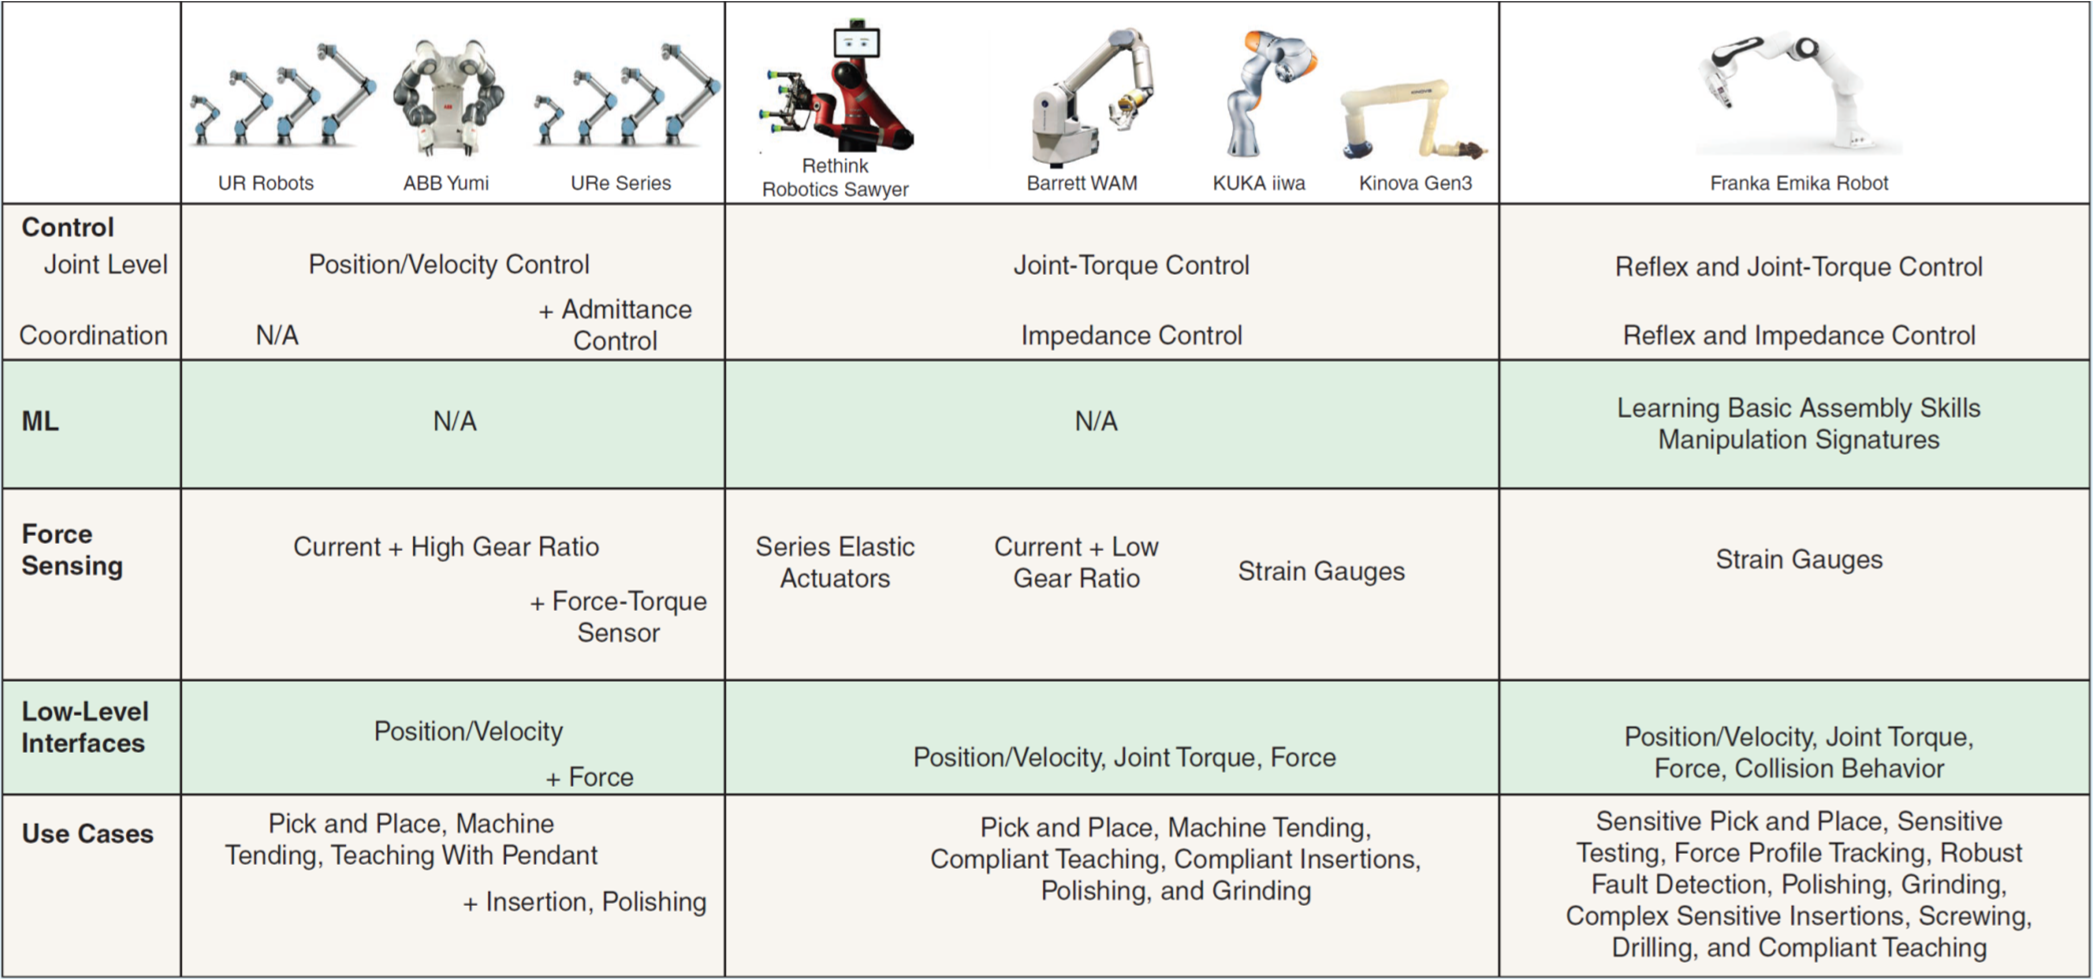
\includegraphics[angle=90,height=0.9\textheight]{figures/related_platforms_comp.png}
    \caption{A technological overview of the most relevant currently available robot manipulators, their control paradigms, sensors, interfaces, and target use cases. The robot images are
taken from \cite{Haddadin.2022,robotsur,robotsyumi,robotswam,robotsiiwa,robotssawyer,kreft2020inverse}. N/A: not applicable; UR: Universal Robot}
    \label{fig:related:platforms:comparison}
\end{figure}



% \begin{table}[]
%     \centering
%     \begin{tabular}{p{1.5cm}|c|c|c|c}
%         Robot & UR Robots, ABB Yumi & URe Series & Rethink Robotics Sawyer, Barret WAM, KUKA iiwa, Kinova Gen3 & \platformname{} \\
%         \hline
%         Joint-level control & Position/velocity control & Position/velocity control & Joint-torque control & Reflex and joint-torque control \\
%         \hline
%         Coordination Control \\ N/A & Admittance control & Impedance control & Reflex and impedance control \\
%         \hline
%         ML & N/A & N/A & N/A & Learning basic assembly skills, manipulation signatures \\ 
%         \hline
%         Force sensing & Current + high gear ratio & Current + high gear ratio, force-torque sensor & Series elastic actuators, current + low gear ratio, strain gauges & Strain gauges\\
%         \hline
%         Low-level interfaces & Position, velocity & Position, velocity, force & position, velocity, joint torque, force & position, velocity, joint torque, force, collision behavior \\
%         \hline
%         Use cases & Pick and place, machine tending, teaching with pendant & Pick and place, machine tending, teaching with pendant, insertion, polishing & Pick and placec, machine tending, compliant teaching, compliant insertion, polishing, grinding & Sensitive pick and place, sensitive testing, force profile tracking, robust fault detection, polishing, grinding, complex sensitive insertion, screwing, drilling, compliant teaching \\
%         \hline
%     \end{tabular}
%     \caption{Caption}
%     \label{tab:my_label}
% \end{table}